

\tikzset{every picture/.style={line width=0.75pt}} %set default line width to 0.75pt        

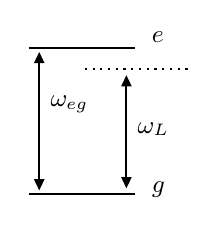
\begin{tikzpicture}[x=0.75pt,y=0.75pt,yscale=-1,xscale=1]
%uncomment if require: \path (0,121); %set diagram left start at 0, and has height of 121

%Straight Lines [id:da16867782903128048] 
\draw  [dash pattern={on 0.8pt off 2.0pt}]  (34,26) -- (84.97,26) ;
%Straight Lines [id:da39705900807308525] 
\draw    (7,86) -- (57.97,86) ;
%Straight Lines [id:da09910835469997958] 
\draw    (12.07,20.73) -- (12.07,81.36) ;
\draw [shift={(12.07,84.36)}, rotate = 270] [fill={rgb, 255:red, 0; green, 0; blue, 0 }  ][line width=0.08]  [draw opacity=0] (5.36,-2.57) -- (0,0) -- (5.36,2.57) -- cycle    ;
\draw [shift={(12.07,17.73)}, rotate = 90] [fill={rgb, 255:red, 0; green, 0; blue, 0 }  ][line width=0.08]  [draw opacity=0] (5.36,-2.57) -- (0,0) -- (5.36,2.57) -- cycle    ;
%Straight Lines [id:da027548097951511363] 
\draw    (7,16) -- (57.97,16) ;
%Straight Lines [id:da21514573737838005] 
\draw    (54.07,31.93) -- (54.07,80.36) ;
\draw [shift={(54.07,83.36)}, rotate = 270] [fill={rgb, 255:red, 0; green, 0; blue, 0 }  ][line width=0.08]  [draw opacity=0] (5.36,-2.57) -- (0,0) -- (5.36,2.57) -- cycle    ;
\draw [shift={(54.07,28.93)}, rotate = 90] [fill={rgb, 255:red, 0; green, 0; blue, 0 }  ][line width=0.08]  [draw opacity=0] (5.36,-2.57) -- (0,0) -- (5.36,2.57) -- cycle    ;

% Text Node
\draw (64.87,6.5) node [anchor=north west][inner sep=0.75pt]  [font=\small]  {$\ket{e}$};
% Text Node
\draw (64.87,78.55) node [anchor=north west][inner sep=0.75pt]  [font=\small]  {$\ket{g}$};
% Text Node
\draw (16,37.39) node [anchor=north west][inner sep=0.75pt]  [font=\small]  {$\omega _{eg}$};
% Text Node
\draw (58,50.19) node [anchor=north west][inner sep=0.75pt]  [font=\small]  {$\omega _{L}$};


\end{tikzpicture}
